\section{Protocol Design} \label{sec:hc-design}

In this section, we describe the components of the HASCHK protocol, step
through each in detail, and then introduce our proof-of-concept implementation
of these components.

\subsection{Participants}

\noindent\textbf{Provider.} The \emph{provider} is the entity in control of both
the server and backend with the goal of ensuring the integrity of resources
downloaded from their system. \\

\noindent\textbf{HASCHK Frontend.} The \emph{frontend} is responsible for
calculating the Uniform Resource Name (URN) and Backend Domain (BD) of the
resource downloaded from the server. Afterwards, the frontend queries the
backend using this URN and, if an integrity violation is detected, quarantines
the resource and warns the user. \\

\noindent\textbf{Server.} The \emph{server} is a distribution system (hopefully)
controlled by the provider that hosts resources for download. It can be internal
or external, a single server or many, first-party or third-party. \\

\noindent\textbf{HASCHK Backend.} The \emph{backend} is responsible for
advertising a queryable listing of URNs that HASCHK frontends can use to
judge the legitimacy of downloads. It is a high availability system that is
wholly separate from the server (not co-hosted) and controlled by the provider.

\subsection{Protocol Overview}

\begin{figure}[ht]
    \centering
    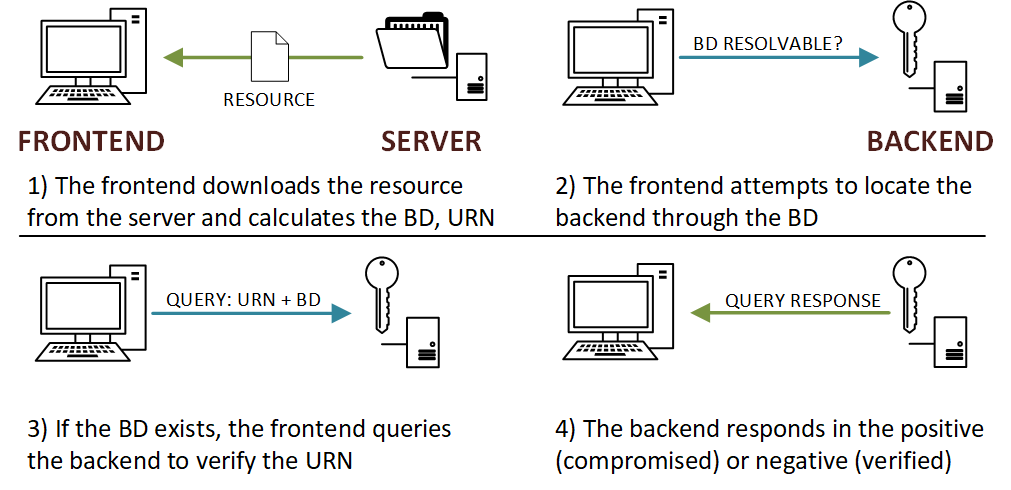
\includegraphics[width=\linewidth]{figs/hc/haschk-overview.png}
    \caption{A high level overview of the (generic) automated checksum
    verification process beginning when a user downloads a
    resource.} \label{fig:protocol}
\end{figure}

\figref{protocol} gives a high level overview of the HASCHK protocol.
Initially, when a user finishes downloading a resource from the provider's
server, the frontend runs the resource's contents through the SHA-256 hashing
function, yielding a 256-bit digest. Any hashing function can be used so long as
it is pre-image and collision resistant~\cite{Rogaway}. This digest is used to
construct a hash-based Uniform Resource Name~\cite{draft-URN} (URN) uniquely identifying the
resource. Additionally, a Backend Domain (BD) is derived from the domain name of
the server. The frontend uses the BD in an implementation-dependent manner to
locate and query the backend, checking for the existence of the constructed URN
and essentially asking: \emph{``is this a compromised resource?''} If the URN is
found, a negative response is returned indicating a verified resource. If the
URN is not found, a positive response is returned indicating a compromised
resource.

If the query returns a positive response: (1) the user should be warned pursuant
to the recommendations of Akhawe et al~\cite{Akhawe} (avoid warning fatigue, be
invisible), Cherubini et al~\cite{Cherubini} (simple non-technical language,
secure default action), Modic et al~\cite{Modic} (issue warnings from a position
of authority), and others; (2) the download should be deleted, renamed, or
otherwise made inaccessible/quarantined by default; and (3) the user should
still be allowed to ``click through'' and override the warning and the default
quarantine behavior, though ideally this should be less convenient than the
default action~\cite{Cherubini}.

If the query returns a negative response, the frontend should indicate this
inconspicuously to mitigate the threat of warning/popup fatigue~\cite{Akhawe,
Cherubini} and habituation~\cite{Sunshine}. For example, our frontend
implementation simply changes its icon when downloads are successfully verified
and only issues popup warnings when compromised downloads are positively
identified.

To prevent false positives, integrity checking is skipped if the backend's
location is unresolvable or HASCHK is not properly deployed. Determining when
this is the case is implementation-dependent. To prevent false-negatives, when
HASCHK is properly deployed and a URN is not found during lookup, the backend
response will always be interpreted as positive. As a result, it is not possible
to only secure ``some'' resources on a server.

\subsubsection{Deriving the Backend Domain (BD)}

Before we can communicate with a provider's backend, we require some scheme to
locate it. We refer to this scheme as \emph{deriving the Backend Domain} (BD).
The BD is some identifier that allows the frontend to locate the backend. For
our Domain Name System (DNS) based implementation (below), the BD is the
Third-Level Subdomain (3LD) or Second-Level Domain (2LD) based on the server
URI's host subcomponent~\cite{RFC3986} and are queried in that order. \\

Example 1: an FTP frontend (\eg{ Filezilla, Transmit, et cetera}) downloading a
resource from an FTP server at
\texttt{ftps://un:pw@ftp.example1.com:8080/some/resource} has a host
subcomponent of \texttt{ftp.example1.com} and a BD of \texttt{ftp.example1.com}
or \texttt{example1.com}. \\

Example 2: a browser frontend (\eg{ Lynx, Google Chrome, Internet Explorer, et
cetera}) downloading a resource at \texttt{https://s4.l.cdn.example2.com/fl}
from a hyperlink on the page \texttt{https://dl.app.example3.com/index/page} has
a host subcomponent of \texttt{dl.app.example3.com} (\emph{not
\texttt{s4.ll.cdn.example2.com}}) and a BD of \texttt{app.example3.com} or
\texttt{example3.com}. \\

It is important that the right BD is derived to ensure correct operation of the
protocol. This concern is implementation-dependent. Specifically, in the case of
the browser frontend in example 2 (above), the BD is not derived from the
resource's URI directly but from the URI of the HTML page containing the
hyperlink pointing to that resource. This prevents an adversary from trivially
fooling HASCHK by, for instance, replacing
\texttt{https://s4.l.cdn.example2.com} with a hyperlink pointing to
\texttt{https://attacker.com} and hosting a conforming HASCHK backend that
would cause the frontend to respond with a false negative.

Further, depending on the implementation, a frontend or backend may not be using
URIs and DNS to transact information over the internet at all. An example of
this is a purely Distributed Hash Table (DHT) based backend. In such a case, any
derivation algorithm (or no derivation at all, \eg{ the BD is hardcoded}) can be
used as long as correct operation of the protocol is ensured.

\subsubsection{Constructing Uniform Resource Names (URN)}

To ensure the integrity of arbitrary resources, we require some method to
uniquely and durably identify those resources. We accomplish this through the
adoption of the informal IETF draft for the construction of hash-based
\emph{Uniform Resource Names} (URNs)~\cite{draft-URN}, which the frontend
follows when calculating URNs for each resource downloaded. Through whatever
implementation-specific method, the backend must ``advertise'' or allow lookups
against a set of expected URNs corresponding to the resources hosted on the
provider's server, even if those resources have unstable access paths or URIs;
\eg{, when resources are hosted externally, on download mirrors, on CDNs, et
cetera}. This requirement is satisfied by implementations combining URNs with
the BD, thus durably associating the URNs calculated in the frontend with the
URNs advertised by a provider's backend regardless of where the corresponding
resources are hosted on the provider's server.

Since the backend advertising URNs is \emph{never} co-hosted alongside the
system that distributes the corresponding resources---like a web or FTP
server---HASCHK retains the ability to protect users from dangerous downloads
\emph{even when the system distributing the resource has been completely
compromised}. This is not true of prior approaches to automated checksum
verification of arbitrary resources~\cite{Cherubini}.
